\documentclass[border=4pt]{standalone}
\usepackage{amsmath,amssymb}
\usepackage{tikz}
\usetikzlibrary{arrows.meta,decorations.pathreplacing}
\begin{document}
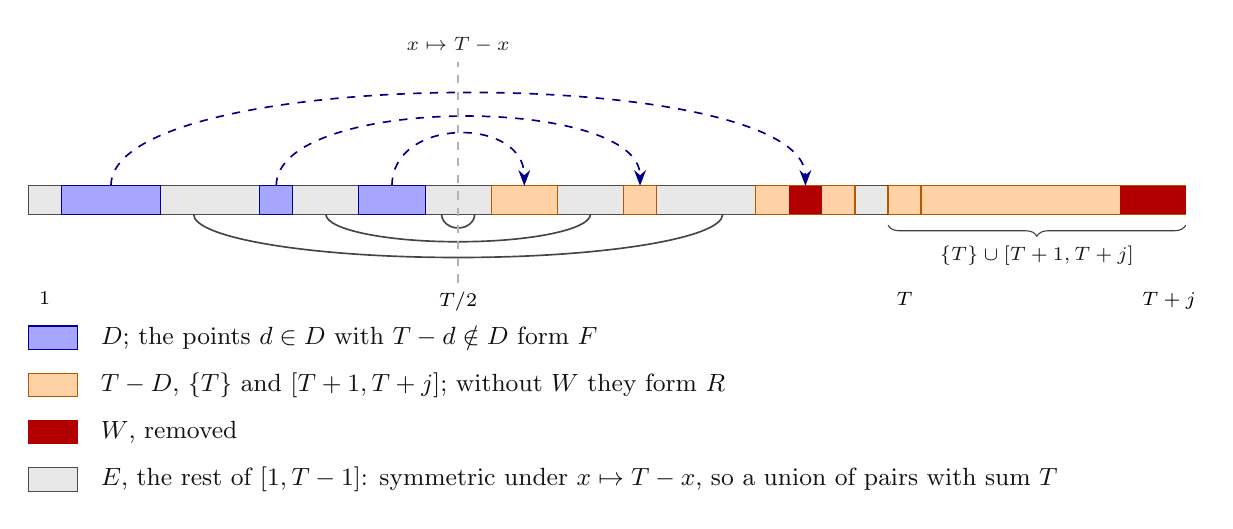
\begin{tikzpicture}[
  x=0.42cm, y=1cm,
  note/.style={font=\small,gray!15!black,align=left,anchor=west},
  tk/.style={font=\scriptsize,anchor=north},
  blk/.style={line width=0.4pt}]
  \def\h{0.18}
  % E: the whole of [1,T-1] first, in gray
  \fill[gray!18] (0.5,-\h) rectangle (26.5,\h);
  \draw[gray!60!black,line width=0.4pt] (0.5,-\h) rectangle (26.5,\h);
  % D (blue) and T-D (orange), mirror images about T/2 = 13.5
  \foreach \u/\v in {1.5/4.5, 7.5/8.5, 10.5/12.5} {
    \fill[blue!35,blk] (\u,-\h) rectangle (\v,\h);
    \draw[blue!60!black,blk] (\u,-\h) rectangle (\v,\h);
    \fill[orange!35] (27-\v,-\h) rectangle (27-\u,\h);
    \draw[orange!70!black,blk] (27-\v,-\h) rectangle (27-\u,\h);
    \draw[-{Stealth[length=2mm]},blue!55!black,dashed,line width=0.6pt]
      ({(\u+\v)/2},\h) .. controls ({(\u+\v)/2},{0.9+0.04*(27-\u-\v)}) and ({27-(\u+\v)/2},{0.9+0.04*(27-\u-\v)}) .. ({27-(\u+\v)/2},\h);
  }
  % T and [T+1, T+j]
  \fill[orange!35] (26.5,-\h) rectangle (35.5,\h);
  \draw[orange!70!black,blk] (26.5,-\h) rectangle (35.5,\h);
  \draw[orange!70!black,line width=0.8pt] (26.5,-\h) -- (26.5,\h);
  \draw[orange!70!black,line width=0.8pt] (27.5,-\h) -- (27.5,\h);
  % W (red): two points at the top and one inside T-D
  \foreach \x in {24,34,35} { \fill[red!70!black] (\x-0.5,-\h) rectangle (\x+0.5,\h); }
  % a few pairs {x, T-x} of E below
  \foreach \x in {5.5,9.5,13} {
    \pgfmathsetmacro{\r}{(27-2*\x)/2}
    \draw[gray!55!black,line width=0.6pt] (\x,-\h) arc[start angle=180,end angle=360,x radius=\r,y radius={0.05*\r+0.15}];
  }
  % mirror axis
  \draw[gray!60,dashed,line width=0.5pt] (13.5,-1.05) -- (13.5,1.75);
  \node[font=\scriptsize,gray!30!black,anchor=south] at (13.5,1.75) {$x\mapsto T-x$};
  % ticks
  \foreach \x/\t in {1/1, 13.5/{T/2}, 27/T, 35/{T+j}} {
    \node[tk] at (\x,-1.05) {$\t$};
  }
  \draw[decorate,decoration={brace,amplitude=4pt,mirror},gray!50!black] (26.5,-0.32) -- (35.5,-0.32)
    node[midway,below=4pt,font=\scriptsize,gray!20!black] {$\{T\}\cup[T+1,T+j]$};
  % legend
  \begin{scope}[yshift=-1.75cm]
    \fill[blue!35] (0.5,-0.15) rectangle (2,0.15); \draw[blue!60!black,blk] (0.5,-0.15) rectangle (2,0.15);
    \node[note] at (2.4,0) {$D$; the points $d\in D$ with $T-d\notin D$ form $F$};
    \fill[orange!35] (0.5,-0.75) rectangle (2,-0.45); \draw[orange!70!black,blk] (0.5,-0.75) rectangle (2,-0.45);
    \node[note] at (2.4,-0.6) {$T-D$, $\{T\}$ and $[T+1,T+j]$; without $W$ they form $R$};
    \fill[red!70!black] (0.5,-1.35) rectangle (2,-1.05);
    \node[note] at (2.4,-1.2) {$W$, removed};
    \fill[gray!18] (0.5,-1.95) rectangle (2,-1.65); \draw[gray!60!black,blk] (0.5,-1.95) rectangle (2,-1.65);
    \node[note] at (2.4,-1.8) {$E$, the rest of $[1,T-1]$: symmetric under $x\mapsto T-x$, so a union of pairs with sum $T$};
  \end{scope}
\end{tikzpicture}
\end{document}
